\chapter{Case study: interface design}
\label{turtlechap}

Code examples from this chapter are available from
\url{http://thinkpython.com/code/polygon.py}.


\section{TurtleWorld}
\label{turtleworld}
\index{TurtleWorld}
\index{Swampy}

To accompany this book, I have written a package called Swampy.
You can download Swampy from \url{http://thinkpython.com/swampy};
follow the instructions there to install Swampy on your system.

A {\bf package} is a collection of modules; one of the modules in
Swampy is {\tt TurtleWorld}, which provides a set of functions for
drawing lines by steering turtles around the screen.
\index{package}

If Swampy is installed as a package on your system, you can import
{\tt TurtleWorld} like this:

\begin{verbatim}
from swampy.TurtleWorld import *
\end{verbatim}

If you downloaded the Swampy modules but did not install them as a
package, you can either work in the directory that contains the Swampy
files, or add that directory to Python's search path.  Then you can import
{\tt TurtleWorld} like this:

\begin{verbatim}
from TurtleWorld import *
\end{verbatim}

The details of the installation process and setting Python's search
path depend on your system, so rather than include those details here,
I will try to maintain current information for several systems
at \url{http://thinkpython.com/swampy}

Create a file named {\tt mypolygon.py} and type in the following
code:

\begin{verbatim}
from swampy.TurtleWorld import *

world = TurtleWorld()
bob = Turtle()
print bob

wait_for_user()
\end{verbatim}
%
The first line imports everything from the {\tt TurtleWorld} module
in the {\tt swampy} package.
\index{import statement}
\index{statement!import}

The next lines create a TurtleWorld assigned to {\tt world} and
a Turtle assigned to {\tt bob}.  Printing {\tt bob} yields something
like:

\begin{verbatim}
<TurtleWorld.Turtle instance at 0xb7bfbf4c>
\end{verbatim}
%
This means that {\tt bob} refers to
an {\bf instance} of a Turtle
as defined in module {\tt TurtleWorld}.  In this context,
``instance'' means a member of a set;
this Turtle is one of the set of possible Turtles.
\index{instance}

\verb"wait_for_user" tells TurtleWorld to wait for the user
to do something, although in this case there's not much for
the user to do except close the window.

TurtleWorld provides several
turtle-steering functions: {\tt fd} and {\tt bk} for
forward and backward, and {\tt lt} and {\tt rt} for left and
right turns.  Also, each Turtle is holding a pen, which is
either down or up; if the pen is down, the Turtle leaves
a trail when it moves.  The functions {\tt pu} and {\tt pd}
stand for ``pen up'' and ``pen down.''

To draw a right angle, add these lines to the program
(after creating {\tt bob} and before calling \verb"wait_for_user"):

\begin{verbatim}
fd(bob, 100)
lt(bob)
fd(bob, 100)
\end{verbatim}
%
The first line tells {\tt bob} to take 100 steps
forward.  The second line tells him to turn left.

When you run this program, you should see {\tt bob} move east and then
north, leaving two line segments behind.

Now modify the program to draw a square.  Don't go on until
you've got it working!

%\newpage

\section{Simple repetition}
\label{repetition}
\index{repetition}

Chances are you wrote something like this (leaving out the code
that creates TurtleWorld and waits for the user):

\begin{verbatim}
fd(bob, 100)
lt(bob)

fd(bob, 100)
lt(bob)

fd(bob, 100)
lt(bob)

fd(bob, 100)
\end{verbatim}
%
We can do the same thing more concisely with a {\tt for} statement.
Add this example to {\tt mypolygon.py} and run it again:
\index{for loop}
\index{loop!for}
\index{statement!for}

\begin{verbatim}
for i in range(4):
    print 'Hello!'
\end{verbatim}
%
You should see something like this:

\begin{verbatim}
Hello!
Hello!
Hello!
Hello!
\end{verbatim}
%
This is the simplest use of the {\tt for} statement; we will see
more later.  But that should be enough to let you rewrite your
square-drawing program.  Don't go on until you do.

Here is a {\tt for} statement that draws a square:

\begin{verbatim}
for i in range(4):
    fd(bob, 100)
    lt(bob)
\end{verbatim}
%
The syntax of a {\tt for} statement is similar to a function
definition.  It has a header that ends with a colon and an indented
body.  The body can contain any number of statements.
\index{loop}

A {\tt for} statement is sometimes called a {\bf loop} because
the flow of execution runs through the body and then loops back
to the top.  In this case, it runs the body four times.

This version is actually a little different from the previous
square-drawing code because it makes another turn after
drawing the last side of the square.  The extra turn takes a little
more time, but it simplifies the code if we do the same thing
every time through the loop.  This version also has the effect
of leaving the turtle back in the starting position, facing in
the starting direction.

\section{Exercises}

The following is a series of exercises using TurtleWorld.  They
are meant to be fun, but they have a point, too.  While you are
working on them, think about what the point is.

The following sections have solutions to the exercises, so
don't look until you have finished (or at least tried).

\begin{enumerate}

\item Write a function called {\tt square} that takes a parameter
named {\tt t}, which is a turtle.  It should use the turtle to draw
a square.

Write a function call that passes {\tt bob} as an argument to
{\tt square}, and then run the program again.

\item Add another parameter, named {\tt length}, to {\tt square}.
Modify the body so length of the sides is {\tt length}, and then
modify the function call to provide a second argument.  Run the
program again.  Test your program with a range of values for {\tt
length}.

\item The functions {\tt lt} and {\tt rt} make 90-degree turns by
default, but you can provide a second argument that specifies the
number of degrees.  For example, {\tt lt(bob, 45)} turns {\tt bob} 45
degrees to the left.

Make a copy of {\tt square} and change the name to {\tt polygon}.  Add
another parameter named {\tt n} and modify the body so it draws an
n-sided regular polygon.  Hint: The exterior angles of an n-sided regular
polygon are $360/n$ degrees.
\index{polygon function}
\index{function!polygon}

\item Write a function called {\tt circle} that takes a turtle, {\tt t},
and radius, {\tt r}, as parameters and that draws an approximate circle
by invoking {\tt polygon} with an appropriate length and number of
sides.  Test your function with a range of values of {\tt r}.
\index{circle function}
\index{function!circle}

Hint: figure out the circumference of the circle and make sure that
{\tt length * n = circumference}.

Another hint: if {\tt bob} is too slow for you, you can speed
him up by changing {\tt bob.delay}, which is the time between moves,
in seconds.  {\tt bob.delay = 0.01} ought to get him moving.

% change this to world.delay

\item Make a more general version of {\tt circle} called {\tt arc}
that takes an additional parameter {\tt angle}, which determines
what fraction of a circle to draw.  {\tt angle} is in units of
degrees, so when {\tt angle=360}, {\tt arc} should draw a complete
circle.
\index{arc function}
\index{function!arc}

\end{enumerate}

\section{Encapsulation}

The first exercise asks you to put your square-drawing code
into a function definition and then call the function, passing
the turtle as a parameter.  Here is a solution:

\begin{verbatim}
def square(t):
    for i in range(4):
        fd(t, 100)
        lt(t)

square(bob)
\end{verbatim}
%
The innermost statements, {\tt fd} and {\tt lt} are
indented twice to show that they are inside the {\tt for} loop,
which is inside the function definition.  The next line,
{\tt square(bob)}, is flush with the left margin, so that is the
end of both the {\tt for} loop and the function definition.

Inside the function, {\tt t} refers to the same turtle {\tt bob}
refers to, so {\tt lt(t)} has the same effect as {\tt lt(bob)}.
So why not call the parameter {\tt bob}?  The idea is that {\tt t}
can be any turtle, not just {\tt bob}, so you could create
a second turtle and pass it as an argument to {\tt square}:

\begin{verbatim}
ray = Turtle()
square(ray)
\end{verbatim}
%
Wrapping a piece of code up in a function is called {\bf
encapsulation}.  One of the benefits of encapsulation is that it
attaches a name to the code, which serves as a kind of documentation.
Another advantage is that if you re-use the code, it is more concise
to call a function twice than to copy and paste the body!
\index{encapsulation}


\section{Generalization}

The next step is to add a {\tt length} parameter to {\tt square}.
Here is a solution:

\begin{verbatim}
def square(t, length):
    for i in range(4):
        fd(t, length)
        lt(t)

square(bob, 100)
\end{verbatim}
%
Adding a parameter to a function is called {\bf generalization}
because it makes the function more general: in the previous
version, the square is always the same size; in this version
it can be any size.
\index{generalization}

The next step is also a generalization.  Instead of drawing
squares, {\tt polygon} draws regular polygons with any number of
sides.  Here is a solution
:rule
\begin{verbatim}
def polygon(t, n, length):
    angle = 360.0 / n
    for i in range(n):
        fd(t, length)
        lt(t, angle)

polygon(bob, 7, 70)
\end{verbatim}
%
This draws a 7-sided polygon with side length 70.  If you have
more than a few numeric arguments, it is easy to forget what they
are, or what order they should be in.  It is legal, and sometimes
helpful, to include the names of the parameters in the argument
list:

\begin{verbatim}
polygon(bob, n=7, length=70)
\end{verbatim}
%
These are called {\bf keyword arguments} because they include
the parameter names as ``keywords'' (not to be confused with
Python keywords like {\tt while} and {\tt def}).
\index{keyword argument}
\index{argument!keyword}

This syntax makes the program more readable.  It is also a reminder
about how arguments and parameters work: when you call a function, the
arguments are assigned to the parameters.


\section{Interface design}

The next step is to write {\tt circle}, which takes a radius,
{\tt r}, as a parameter.  Here is a simple solution that uses
{\tt polygon} to draw a 50-sided polygon:

\begin{verbatim}
def circle(t, r):
    circumference = 2 * math.pi * r
    n = 50
    length = circumference / n
    polygon(t, n, length)
\end{verbatim}
%
The first line computes the circumference of a circle with radius
{\tt r} using the formula $2 \pi r$.  Since we use {\tt math.pi}, we
have to import {\tt math}.  By convention, {\tt import} statements
are usually at the beginning of the script.

{\tt n} is the number of line segments in our approximation of a circle,
so {\tt length} is the length of each segment.  Thus, {\tt polygon}
draws a 50-sides polygon that approximates a circle with radius {\tt r}.

One limitation of this solution is that {\tt n} is a constant, which
means that for very big circles, the line segments are too long, and
for small circles, we waste time drawing very small segments.  One
solution would be to generalize the function by taking {\tt n} as
a parameter.  This would give the user (whoever calls {\tt circle})
more control, but the interface would be less clean.
\index{interface}

The {\bf interface} of a function is a summary of how it is used: what
are the parameters?  What does the function do?  And what is the return
value?  An interface is ``clean'' if it is ``as simple as
possible, but not simpler. (Einstein)''
\index{Einstein, Albert}

In this example, {\tt r} belongs in the interface because it
specifies the circle to be drawn.  {\tt n} is less appropriate
because it pertains to the details of {\em how} the circle should
be rendered.

Rather than clutter up the interface, it is better
to choose an appropriate value of {\tt n}
depending on {\tt circumference}:

\begin{verbatim}
def circle(t, r):
    circumference = 2 * math.pi * r
    n = int(circumference / 3) + 1
    length = circumference / n
    polygon(t, n, length)
\end{verbatim}
%
Now the number of segments is (approximately) {\tt circumference/3},
so the length of each segment is (approximately) 3, which is small
enough that the circles look good, but big enough to be efficient,
and appropriate for any size circle.


\section{Refactoring}
\label{refactoring}
\index{refactoring}

When I wrote {\tt circle}, I was able to re-use {\tt polygon}
because a many-sided polygon is a good approximation of a circle.
But {\tt arc} is not as cooperative; we can't use {\tt polygon}
or {\tt circle} to draw an arc.

One alternative is to start with a copy
of {\tt polygon} and transform it into {\tt arc}.  The result
might look like this:

\begin{verbatim}
def arc(t, r, angle):
    arc_length = 2 * math.pi * r * angle / 360
    n = int(arc_length / 3) + 1
    step_length = arc_length / n
    step_angle = float(angle) / n

    for i in range(n):
        fd(t, step_length)
        lt(t, step_angle)
\end{verbatim}
%
The second half of this function looks like {\tt polygon}, but we
can't re-use {\tt polygon} without changing the interface.  We could
generalize {\tt polygon} to take an angle as a third argument,
but then {\tt polygon} would no longer be an appropriate name!
Instead, let's call the more general function {\tt polyline}:

\begin{verbatim}
def polyline(t, n, length, angle):
    for i in range(n):
        fd(t, length)
        lt(t, angle)
\end{verbatim}
%
Now we can rewrite {\tt polygon} and {\tt arc} to use {\tt polyline}:

\begin{verbatim}
def polygon(t, n, length):
    angle = 360.0 / n
    polyline(t, n, length, angle)

def arc(t, r, angle):
    arc_length = 2 * math.pi * r * angle / 360
    n = int(arc_length / 3) + 1
    step_length = arc_length / n
    step_angle = float(angle) / n
    polyline(t, n, step_length, step_angle)
\end{verbatim}
%
Finally, we can rewrite {\tt circle} to use {\tt arc}:

\begin{verbatim}
def circle(t, r):
    arc(t, r, 360)
\end{verbatim}
%
This process---rearranging a program to improve function
interfaces and facilitate code re-use---is called {\bf refactoring}.
In this case, we noticed that there was similar code in {\tt arc} and
{\tt polygon}, so we ``factored it out'' into {\tt polyline}.
\index{refactoring}

If we had planned ahead, we might have written {\tt polyline} first
and avoided refactoring, but often you don't know enough at the
beginning of a project to design all the interfaces.  Once you start
coding, you understand the problem better.  Sometimes refactoring is a
sign that you have learned something.


\section{A development plan}
\index{development plan!encapsulation and generalization}

A {\bf development plan} is a process for writing programs.
The process we used
in this case study is ``encapsulation and
generalization.''  The steps of this process are:

\begin{enumerate}

\item Start by writing a small program with no function definitions.

\item Once you get the program working, encapsulate it in a function
and give it a name.

\item Generalize the function by adding appropriate parameters.

\item Repeat steps 1--3 until you have a set of working functions.
Copy and paste working code to avoid retyping (and re-debugging).

\item Look for opportunities to improve the program by refactoring.
For example, if you have similar code in several places, consider
factoring it into an appropriately general function.

\end{enumerate}

This process has some drawbacks---we will see alternatives later---but
it can be useful if you don't know ahead of time how to divide the
program into functions.  This approach lets you design as you go
along.


\section{docstring}
\label{docstring}
\index{docstring}

A {\bf docstring} is a string at the beginning of a function that
explains the interface (``doc'' is short for ``documentation'').  Here
is an example:

\begin{verbatim}
def polyline(t, n, length, angle):
    """Draws n line segments with the given length and
    angle (in degrees) between them.  t is a turtle.
    """
    for i in range(n):
        fd(t, length)
        lt(t, angle)
\end{verbatim}
%
This docstring is a triple-quoted string, also known
as a multiline string because the triple quotes allow the string
to span more than one line.
\index{quotation mark}
\index{triple-quoted string}
\index{string!triple-quoted}
\index{multiline string}
\index{string!multiline}

It is terse, but it contains the essential information
someone would need to use this function.  It explains concisely what
the function does (without getting into the details of how it does
it).  It explains what effect each parameter has on the behavior of
the function and what type each parameter should be (if it is not
obvious).

Writing this kind of documentation is an important part of interface
design.  A well-designed interface should be simple to explain;
if you are having a hard time explaining one of your functions,
that might be a sign that the interface could be improved.


\section{Debugging}
\index{debugging}
\index{interface}

An interface is like a contract between a function and a caller.
The caller agrees to provide certain parameters and the function
agrees to do certain work.

For example, {\tt polyline} requires four arguments: {\tt t} has to be
a Turtle; {\tt n} is the number of line segments, so it has to be an
integer; {\tt length} should be a positive number; and {\tt
  angle} has to be a number, which is understood to be in degrees.

These requirements are called {\bf preconditions} because they
are supposed to be true before the function starts executing.
Conversely, conditions at the end of the function are
{\bf postconditions}.  Postconditions include the intended
effect of the function (like drawing line segments) and any
side effects (like moving the Turtle or making other changes
in the World).
\index{precondition}
\index{postcondition}

Preconditions are the responsibility of the caller.  If the caller
violates a (properly documented!) precondition and the function
doesn't work correctly, the bug is in the caller, not the function.

% Removing this because we haven't seen conditionals yet!
%However, for purposes of debugging it is often a good idea for
%functions to check their preconditions rather than assume they are
%true.  If every function checks its preconditions before starting,
%then if something goes wrong, you will know which function to blame.


\section{Glossary}

\begin{description}

\item[instance:] A member of a set.  The TurtleWorld in this
chapter is a member of the set of TurtleWorlds.
\index{instance}

\item[loop:] A part of a program that can execute repeatedly.
\index{loop}

\item[encapsulation:] The process of transforming a sequence of
statements into a function definition.
\index{encapsulation}

\item[generalization:] The process of replacing something
unnecessarily specific (like a number) with something appropriately
general (like a variable or parameter).
\index{generalization}

\item[keyword argument:] An argument that includes the name of
the parameter as a ``keyword.''
\index{keyword argument}
\index{argument!keyword}

\item[interface:] A description of how to use a function, including
the name and descriptions of the arguments and return value.
\index{interface}

\item[refactoring:] The process of modifying a working program to
  improve function interfaces and other qualities of the code.
\index{refactoring}

\item[development plan:] A process for writing programs.
\index{development plan}

\item[docstring:]  A string that appears in a function definition
to document the function's interface.
\index{docstring}

\item[precondition:] A requirement that should be satisfied by
the caller before a function starts.
\index{precondition}

\item[postcondition:] A requirement that should be satisfied by
the function before it ends.
\index{precondition}

\end{description}


\section{Exercises}

\begin{exercise}

Download the code in this chapter from
\url{http://thinkpython.com/code/polygon.py}.

\begin{enumerate}

\item Write appropriate docstrings for {\tt polygon}, {\tt arc} and
{\tt circle}.
\index{stack diagram}

\item Draw a stack diagram that shows the state of the program
while executing {\tt circle(bob, radius)}.  You can do the
arithmetic by hand or add {\tt print} statements to the code.

\item The version of {\tt arc} in Section~\ref{refactoring} is not
very accurate because the linear approximation of the
circle is always outside the true circle.  As a result,
the turtle ends up a few units away from the correct
destination. My solution shows a way to reduce
the effect of this error.  Read the code and see if it makes
sense to you.  If you draw a diagram, you might see how it works.

\end{enumerate}

\end{exercise}

\begin{figure}
\centerline
{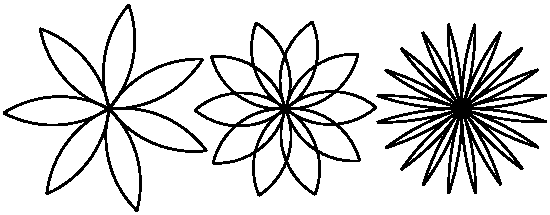
\includegraphics[scale=0.8]{figs/flowers.pdf}}
\caption{Turtle flowers.}
\label{fig.flowers}
\end{figure}

\begin{exercise}
\index{flower}

Write an appropriately general set of functions that
can draw flowers as in Figure~\ref{fig.flowers}.

Solution: \url{http://thinkpython.com/code/flower.py},
also requires \url{http://thinkpython.com/code/polygon.py}.

\end{exercise}

\begin{figure}
\centerline
{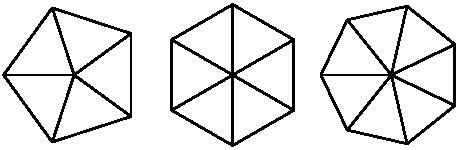
\includegraphics[scale=0.8]{figs/pies.pdf}}
\caption{Turtle pies.}
\label{fig.pies}
\end{figure}


\begin{exercise}
\index{pie}

Write an appropriately general set of functions that
can draw shapes as in Figure~\ref{fig.pies}.

Solution: \url{http://thinkpython.com/code/pie.py}.

\end{exercise}

\begin{exercise}
\index{alphabet}
\index{turtle typewriter}
\index{typewriter, turtle}

The letters of the alphabet can be constructed from a moderate number
of basic elements, like vertical and horizontal lines and a few
curves.  Design a font that can be drawn with a minimal number of
basic elements and then write functions that draw letters of the
alphabet.

You should write one function for each letter, with names
\verb"draw_a", \verb"draw_b", etc., and put your functions
in a file named {\tt letters.py}.  You can download a
``turtle typewriter'' from \url{http://thinkpython.com/code/typewriter.py}
to help you test your code.

Solution: \url{http://thinkpython.com/code/letters.py}, also requires
\url{http://thinkpython.com/code/polygon.py}.

\end{exercise}

\begin{exercise}

Read about spirals at \url{http://en.wikipedia.org/wiki/Spiral}; then
write a program that draws an Archimedian spiral (or one of the other
kinds).  Solution: \url{http://thinkpython.com/code/spiral.py}.
\index{spiral}
\index{Archimedian spiral}

\end{exercise}
